\documentclass[titlepage,11pt, oneside]{article}   	% use "amsart" instead of "article" for AMSLaTeX format
\usepackage{geometry}                		% See geometry.pdf to learn the layout options. There are lots.
\usepackage[utf8]{inputenc}
\geometry{letterpaper}                   		% ... or a4paper or a5paper or ... 
%\geometry{landscape}                		% Activate for rotated page geometry
%\usepackage[parfill]{parskip}    		% Activate to begin paragraphs with an empty line rather than an indent
\usepackage{graphicx}				% Use pdf, png, jpg, or eps§ with pdflatex; use eps in DVI mode
								% TeX will automatically convert eps --> pdf in pdflatex		
\usepackage{amssymb}
\usepackage{authblk}
\usepackage{indentfirst}
\usepackage{gensymb}
\usepackage{hyperref}
\usepackage[labelfont=bf]{caption}
%SetFonts
\makeatletter
\renewcommand{\maketitle}{\bgroup\setlength{\parindent}{0pt}
\begin{flushleft}
  \textbf{\@title}

  \@author
\end{flushleft}\egroup
}
\makeatother

\title{\textbf{Complete chloroplast genome sequence of a white spruce (\textit{Picea glauca}) genotype from eastern Canada\newline}}

\author[a]{Diana Lin}
\author[a]{Lauren Coombe}
\author[a]{Shaun D. Jackman}
\author[a]{Kristina K. Gagalova}
\author[a]{René L. Warren}
\author[a*]{S. Austin Hammond}
\author[a]{Heather Kirk}
\author[a]{Pawan Pandoh}
\author[a]{Yongjun Zhao}
\author[a]{Richard A. Moore}
\author[a]{Andrew J. Mungall}
\author[b,f]{Carol Ritland}
\author[c]{Barry Jaquish}
\author[d]{Nathalie Isabel}
\author[e]{Jean Bousquet}
\author[a]{Steven J.M. Jones}
\author[b,f]{Joerg Bohlmann}
\author[a]{Inanc Birol}

\affil[a]{Canada's Michael Smith Genome Sciences Centre, BC Cancer, Vancouver, BC, Canada}

\affil[b]{Department of Forest and Conservation Sciences, University of British Columbia, Vancouver, BC, Canada}

\affil[c]{British Columbia Ministry of Forests, Lands and Natural Resource Operations, Tree Improvement Branch, Kalamalka Forestry Centre, Vernon, BC, Canada}

\affil[d]{Natural Resources Canada, Laurentian Forestry Centre, Quebec City, QC, Canada}
\affil[e]{Canada Research Chair in Forest Genomics, Université Laval, Quebec City, QC, Canada}
\affil[f]{Michael Smith Laboratories, University of British Columbia, Vancouver, BC Canada}

\date{April 3, 2019}					% Activate to display a given date or no date

\begin{document}
\maketitle

\noindent Running Head: Complete chloroplast genome of a \textit{Picea glauca} isolate\newline

\noindent \#Address correspondence to Inanc Birol, \href{mailto:ibirol@bcgsc.ca}{ibirol@bcgsc.ca}\newline

\noindent *Current address: S. Austin Hammond, Next-Generation Sequencing Facility, University of Saskatchewan, Saskatoon, SK, Canada.


\begin{abstract}

Here we present the complete chloroplast genome sequence of white spruce (\textit{Picea glauca}, isolate WS77111), a coniferous tree widespread in the boreal forests of North America. This sequence contributes to genomic and phylogenetic analyses of the \textit{Picea} genus, part of ongoing research to understand their adaptation to environmental stress.

\end{abstract}

\section*{Genome Announcement}

We sequenced, assembled, and annotated the chloroplast genome of white spruce (\textit{Picea glauca} genotype WS77111), a dominant species in the Canadian boreal forest (1). Over tens of millions of years, conifers such as \textit{P. glauca} have evolved to cope with adverse environmental conditions (2). However, climate change poses new challenges to the capacity of these trees to adapt to conditions such as prolonged drought and increased pressure from forest insect pests (3). \textit{P. glauca} has three different genomes, a nuclear genome, a mitochondrial genome, and a plastid (i.e. chloroplast) genome. In general, chloroplast genomes are derived from the ancestral genomes of the microbial endosymbiont from which these organelles originated (4). The nuclear genome of \textit{P. glauca} (WS77111) was published in 2015 (5).
\newline
\par
A \textit{P. glauca} (genotype WS77111) needle tissue sample was collected in southeastern Ontario (44\degree19'48"N, 78\degree9'0"W; elevation: 250m). The sample was sequenced at Canada’s Michael Smith Genome Sciences Centre (GSC).
\newline
\par
To sequence the sample, genomic DNA libraries were constructed according to GSC plate-based and paired-end library protocols on a Microlab NIMBUS liquid handling robot (Hamilton, USA), and sonicated into 400 bp fragments, as previously described (6-7). Pooled libraries were sequenced with paired-end 250 bp reads on an Illumina HiSeq2500 instrument in rapid mode.
\newline
\par
To assemble the chloroplast genome, we generated various random subsamples of the full read set (0.75, 1.5, 3, 6, 12, 25, 50, 200 million read pairs), and assembled each subset with ABySS v2.1.0 (8) ($k=128$, $kc=3$). The 1.5M, 3M, and 6M read subsets produced the best ABySS chloroplast genome assemblies (\textit{N\textsubscript{50}} = 3692, 1313, 949, respectively), as determined by comparing these assemblies to the white spruce admix (PG29) chloroplast genome (NCBI accession \href{https://www.ncbi.nlm.nih.gov/nuccore/NC_028594.1}{NC\_028594.1}; (9)) using QUAST v5.0.0 (10). We then performed additional ABySS assemblies with varying k and kc parameters using these three subsets ($k=96, 112, 128, 144, 160, kc=3, 4$). The assembly with the fewest aligning contigs ($n=14$) and fewest misassemblies (1.5M read pairs, $k=96, kc=3$) was chosen for further scaffolding. Scaffolding the assembly using LINKS v1.8.5 (11) and the PG29 chloroplast genome joined the contigs into one piece. We then used Sealer (12) to close the scaffold gaps.We modified the start position of our assembly to match the PG29 reference using BLAST v.2.7.1 (13), and polished the final assembly with Pilon v1.22 (14).
\newline
\par
The complete WS77111 chloroplast genome is 123,421 bp long, with 38.74\% GC content. Using GeSeq (15) with several other \textit{Picea} chloroplast genomes as reference (9, 16), we annotated 114 genes: 74 protein-coding, 36 tRNA-coding, and four rRNA-coding genes. Only \textit{rps12, petB, petD, rpl16,} and \textit{psbZ} required manual annotation. The genome map in Figure \ref{fig:ogdraw} was generated using OGDRAW v1.2 (17).
\newline
\par
The assembly of this new chloroplast genome will enable further analysis of \textit{Picea} phylogeny and genetics.
\newline
\newline
\textbf{Accession number(s).} The complete chloroplast genome sequence of \textit{Picea glauca}, genotype WS77111 is available from Genbank under accession \href{https://www.ncbi.nlm.nih.gov/nuccore/MK174379}{MK174379}, and the raw reads are in the SRA under \href{https://www.ncbi.nlm.nih.gov/sra/SRX525336}{SRX525336}. The annotations used as references were from Picea abies (\href{https://www.ncbi.nlm.nih.gov/nuccore/NC_021456}{NC\_021456}), Picea asperata (\href{https://www.ncbi.nlm.nih.gov/nuccore/NC_032367}{NC\_032367}), Picea glauca genotype PG29 (\href{https://www.ncbi.nlm.nih.gov/nuccore/NC_028594}{NC\_028594}), Picea morrisonicola (\href{https://www.ncbi.nlm.nih.gov/nuccore/NC_016069}{NC\_016069}), and Picea sitchensis (\href{https://www.ncbi.nlm.nih.gov/nuccore/NC_011152}{NC\_011152}, \href{https://www.ncbi.nlm.nih.gov/nuccore/KU215903}{KU215903}).

\section*{Figures and Data}
\begin{figure}[h]
\centering
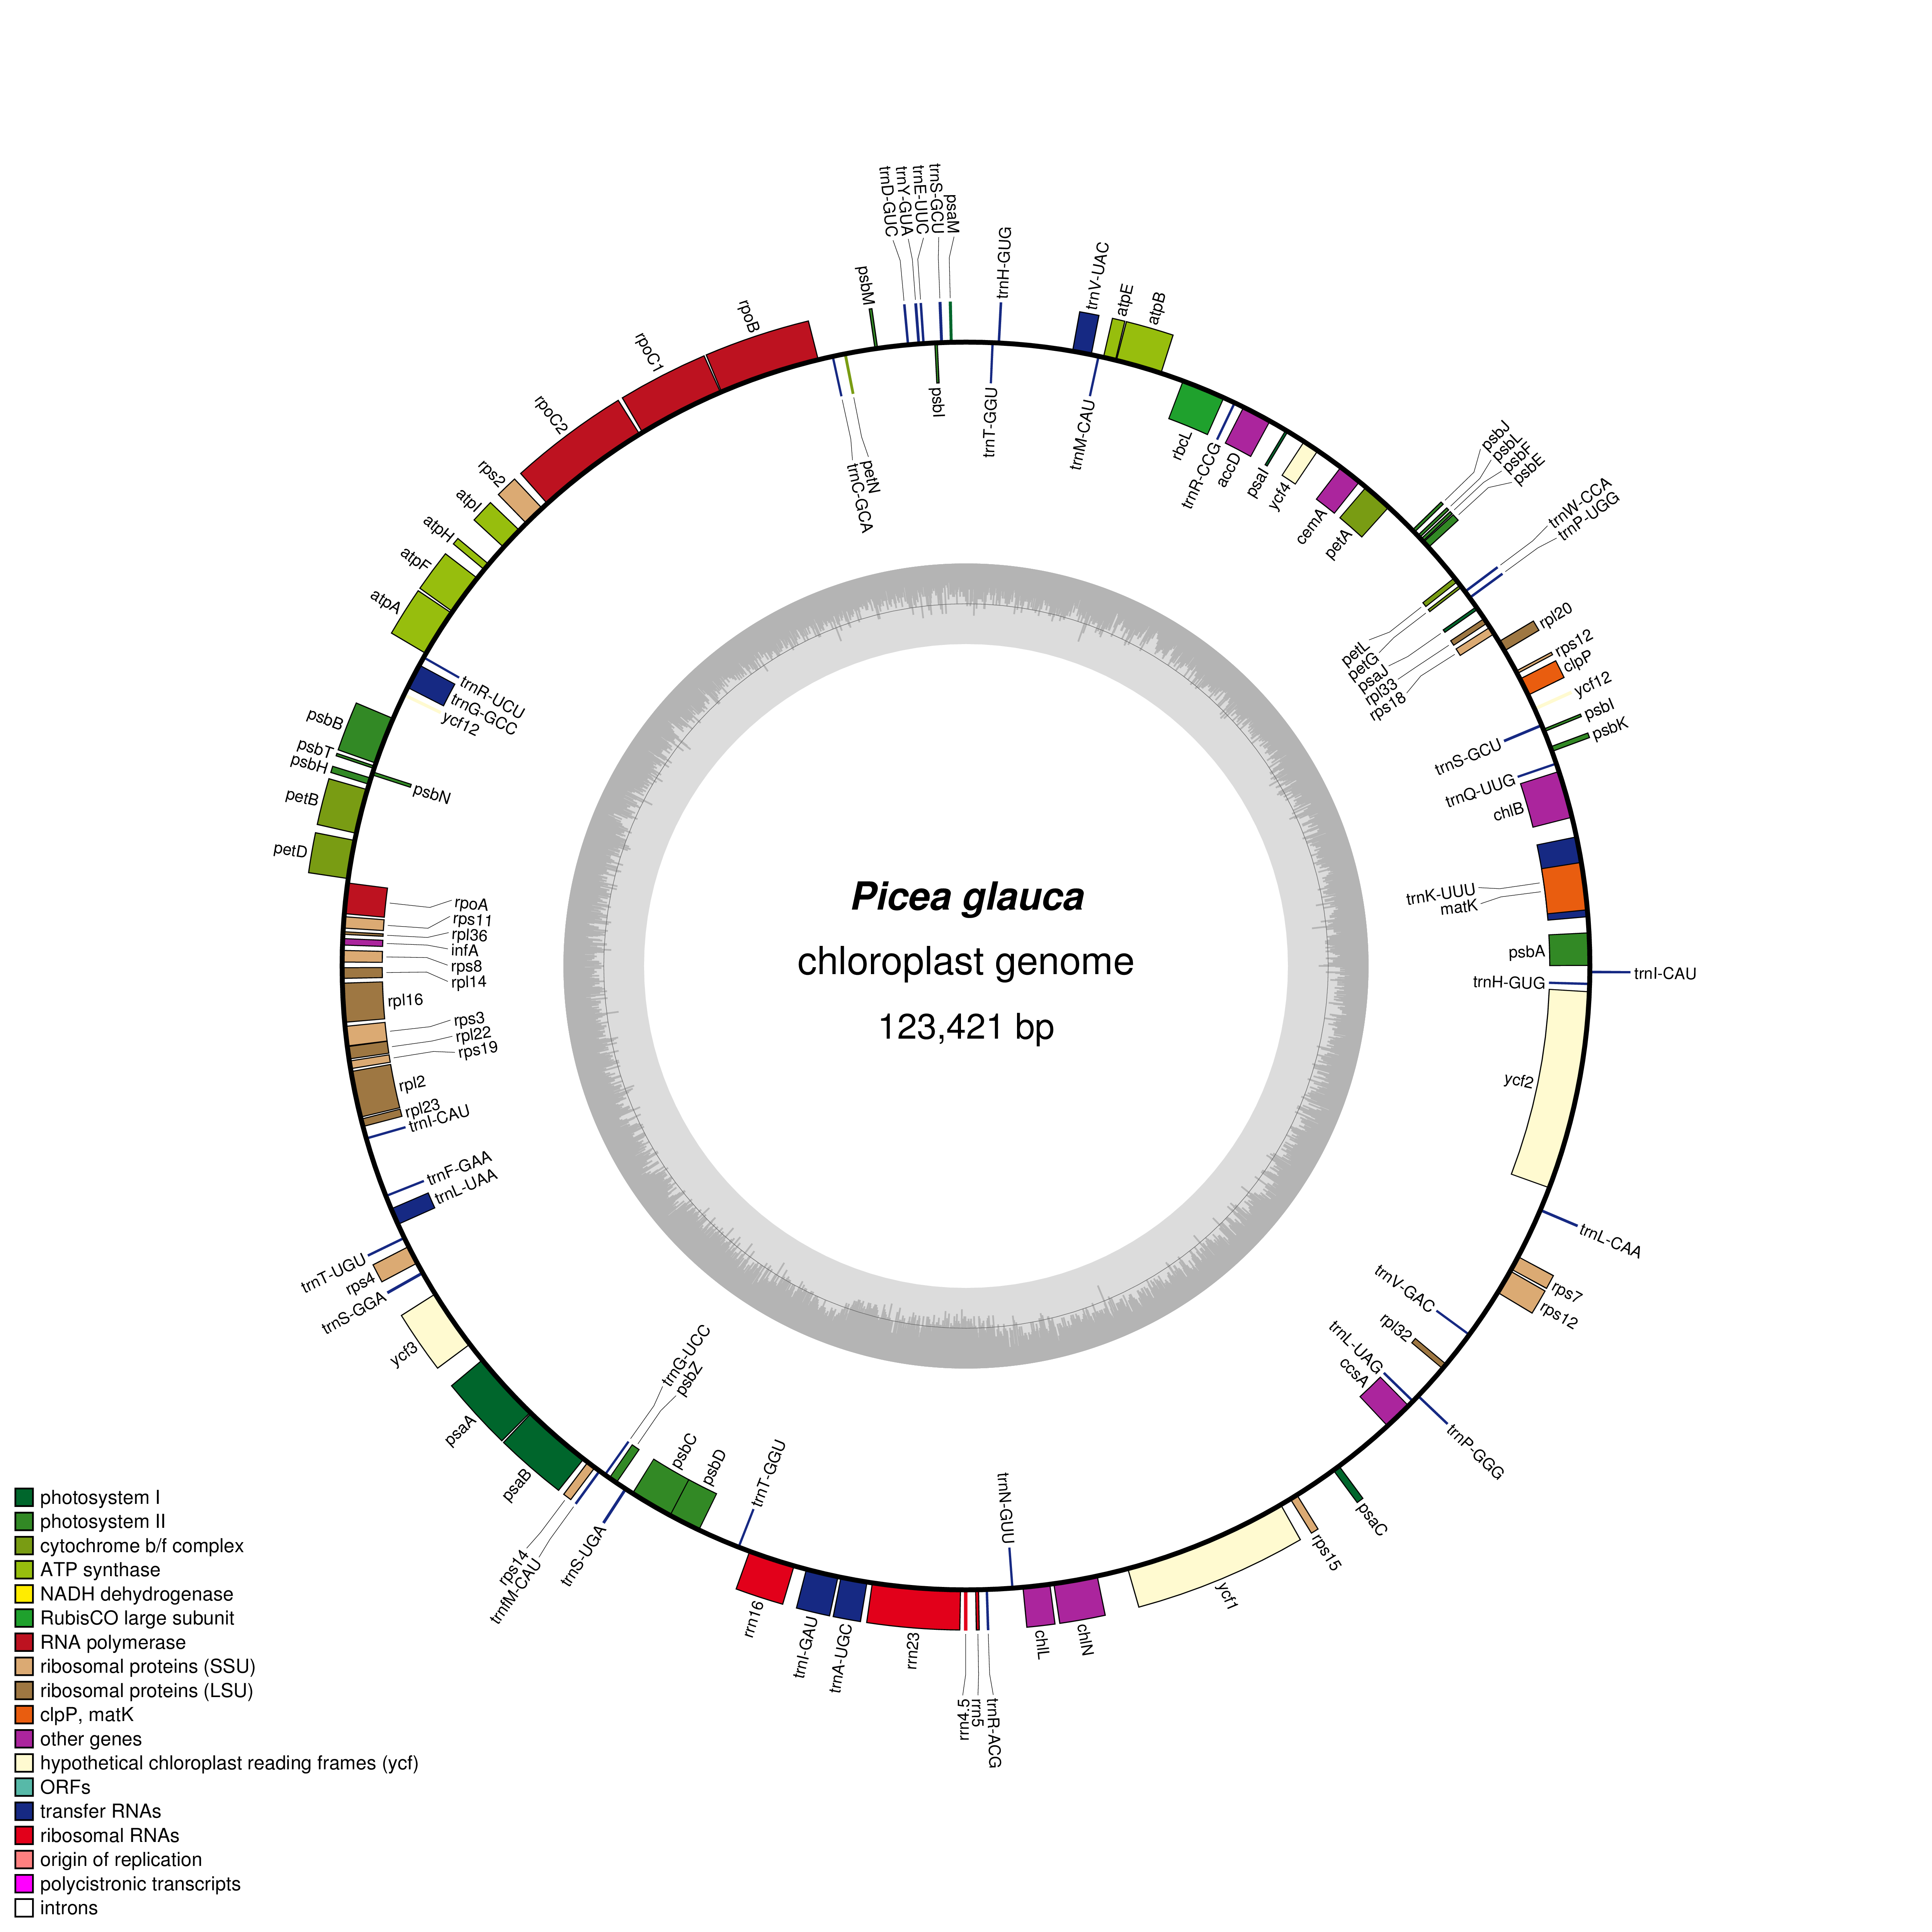
\includegraphics[width=0.72\textwidth]{WS77111}
\caption{\textbf{The complete chloroplast genome of \textit{Picea glauca}, isolate WS77111.} The \textit{Picea glauca} chloroplast genome was annotated using GeSeq (15), and plotted using OGDRAW (17). The inner grey circle illustrates the GC content of the genome.}
\label{fig:ogdraw}
\end{figure}

\section*{Acknowledgements}
This work was supported by funds from Genome Canada, Genome BC, and Genome Quebec as part of the Spruce-Up (\url{www.spruce-up.ca}) [243FOR] and AnnoVis [281ANV] projects.

\section*{References}

\begin{enumerate}
\item  Li P, Beaulieu J, Bousquet J. 1997. Genetic structure and patterns of genetic variation among populations in eastern white spruce (\textit{Picea glauca}). Can J For Res 27:189-198.
\item Bouillé M, Bousquet J. 2005. Trans-species shared polymorphisms at orthologous nuclear gene loci among distant species in the conifer \textit{Picea} (\textit{Pinaceae}): implications for the long-term maintenance of genetic diversity in trees. Am J Bot 92:63-73
\item Kiss GK, Yanchuk AD. 1991. Preliminary evaluation of genetic variation of weevil resistance in interior spruce in British Columbia. Can J For Res 21:230–234.
\item Ku C, Nelson-Sathi S, Roettger M, Sousa FL, Lockhart PJ, Bryant D, Hazkani-Covo E, McInerney JO, Landan G, Martin WF. 2015. Endosymbioitic origin and differential loss of eukaryotic genes. Nature 524:427-432.
\item Warren RL, Keeling CI, Yuen MMS, Raymond A, Taylor GA, Vandervalk BP, Mohamadi H, Paulino D, Chiu R, Jackman SD, Robertson G, Yang C, Boyle B, Hoffmann M, Weigel D, Nelson DR, Ritland C, Isabel N, Jaquish B, Yanchuk A, Bousquet J, Jones SJM, Mackay J, Birol I, Bohlmann J. 2015. Improved white spruce (\textit{Picea glauca}) genome assemblies and annotation of large gene families of conifer terpenoid and phenolic defense metabolism. Plant J 83:189-212
\item Jones MR, Schrader KA, Shen Y, Pleasance E, Chng C, Dar N, Yip S, Renouf DJ, Schein JE, Mungall AJ, Zhao Y, Moore R, Ma Y, Sheffield BS, Ng T, Jones SJM, Marra MA, Laskin J, Lim HJ. 2016. Response to angiotensin blockade with irbesartan in a patient with metastatic colorectal cancer. Ann Oncol 27:801–806.
\item Tsang ES, Shen Y, Chooback N, Ho C, Jones M, Renouf DJ, Lim HJ, Sun S, Yip S, Pleasance E, Ma Y, Zhao Y, Mungall AJ, Moore R, Jones S, Marra M, Laskin JJ. 2017. Clinical outcomes after whole genome sequencing in patients with metastatic non-small cell lung cancer. J Clin Oncol 35.
\item Jackman SD, Vandervalk BP, Mohamadi H, Chu J, Yeo S, Hammond SA, Jahesh G, Khan H, Coombe L, Warren RL, Birol I. 2017. ABySS 2.0: resource-efficient assembly of large genomes using a Bloom filter. Genome Res 27:768-777.
\item Jackman SD, Warren RL, Gibb EA, Vandervalk BP, Mohamadi H, Chu J, Raymond A, Pleasance S, Coope R, Wildung MR, Ritland CE, Bousquet J, Jones SJM, Bohlmann J, Birol I. 2016. Organellar genomes of white spruce (Picea glauca): Assembly and annotation. Genome Biol Evol 8:29–41.
\item Mikheenko A, Prjibelski A, Saveliev V, Antipov D, Gurevich A. 2018. Versatile genome assembly evaluation with QUAST-LG. Bioinformatics 34:i142–i150.
\item Warren RL, Yang C, Vandervalk BP, Behsaz B, Lagman A, Jones SJM, Birol I. 2015. LINKS: Scalable, alignment-free scaffolding of draft genomes with long reads. Gigascience 4:35-35.
\item Paulino D, Warren RL, Vandervalk BP, Raymond A, Jackman SD, Birol I. 2015. Sealer: a scalable gap-closing application for finishing draft genomes. BMC Bioinformatics 16.
\item Altschul SF, Gish W, Miller W, Myers EW, Lipman DJ. 1990. Basic local alignment search tool. J Mol Biol 215:403-410.
\item Walker BJ, Abeel T, Shea T, Priest M, Abouelliel A, Sakthikumar S, Cuomo CA, Zeng Q, Wortman J, Young SK, Earl AM. 2014. Pilon: an integrated tool for comprehensive microbial variant detection and genome assembly improvement. PloS One 9:e112963-e112963.
\item Tillich M, Lehwark P, Pellizzer T, Ulbricht-Jones ES, Fischer A, Bock R, Greiner S. 2017. GeSeq – versatile and accurate annotation of organelle genomes. Nucleic Acids Res 45.
\item Coombe L, Warren RL, Jackman SD, Yang C, Vandervalk BP, Moore RA, Pleasance S, Coope RJ, Bohlmann J, Holt RA, Jones SJM, Birol I. 2016. Assembly of the complete Sitka spruce chloroplast genome using 10X Genomics’ GemCode sequencing data. PLoS One 11.
\item Lohse M, Drechsel O, Kahlau S, Bock R. 2013. OrganellarGenomeDRAW--a suite of tools for generating physical maps of plastid and mitochondrial genomes and visualizing expression data sets. Nucleic Acids Res 41:W575-W581.
\end{enumerate}

\end{document}  